\subsubsection{Serial}
Die serielle Datenübertragung wird per UART realisiert. Das Pixhawk besitzt fünf serielle Interfaces. Einige dieser sind bereits reserviert, z.B. das GPS. Drei Interfaces stehen für die Entwickler zur Verfügung, AMC0 (USB Anschluss), ttyS5 (Serial 4) und ttyS6 (Serial5). Diese Bezeichnungen basieren auf GNU/Linux. Auf AMC0 und ttyS5 sind bereits belegt durch eine nsh. Die Implementation der Lese- und Schreib-Methode sind nicht reentrent. Deshalb sollte die Schnittstelle nur von einem Thread verwendet werden. Aus diesem Grund wurde \textbf{ttyS6} für den Datenstrom verwendet, damit keine anderen App das Interface belegt.\\ 

\noindent Auf der Host Seite wird ein USB $\leftrightarrow$ UART Konverter verwendet. Für diese PAIND Arbeit wurde ein offizielles FTDI Kabel verwendet. Je nach Anschluss (siehe Abbildung \ref{fig:Serielle Schnitstelle} ) wird eine andere Schnittstelle verwendet. Für diese Arbeit wurde ttyS6 belegt.


\begin{figure}[ht]
	\begin{center}
		\begin{subfigure}{0.49\textwidth}
%			\begin{center}
  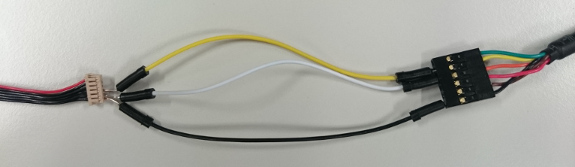
\includegraphics[scale=0.5]{pic/50_app/ttyS5_hw.jpg}
  \caption{ttyS5 mit nsh}
  \label{fig:ttyS5_cable}
%		\end{center}
		\end{subfigure}
		
		\begin{subfigure}{0.49\textwidth}
%		\begin{center}
  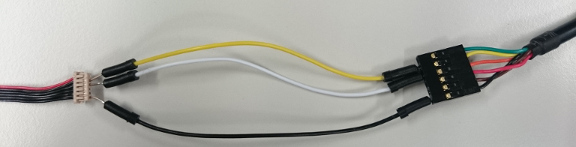
\includegraphics[scale=0.5]{pic/50_app/ttyS6_hw.jpg}
  \caption{ttyS6 ohne nsh}
  \label{fig:ttyS6_cable}
%		\end{center}
		\end{subfigure}
		
		\caption{Serielle Schnitstelle}
		\label{fig:Serielle Schnitstelle}
	\end{center}
\end{figure}


\noindent Anbei die Farbcodierung der Signalleitungen:
\begin{table}[ht]
\begin{center}
  \begin{tabular}{| c | c | c |}
    \hline
    Farbe & Verwendung Pixhawk & Verwendung Host PC \\
    \hline
    gelb  & TX & RX \\
    \hline
    weiss & RX & TX \\
    \hline
    schwarz & GND & GND \\
    \hline
  \end{tabular}
  
  \caption{UART Farbcodierung}
  \label{tab:UART color}
  
\end{center}
\end{table}

\paragraph{Baud}\mbox{}\\
\noindent Das uORB Datenpaket 'Sensor combined' enthält 722 Bytes. Dies könnte eine hohe Bandbreite erfordern. Es ist nicht genau klar, wie oft dieses in der uORB bereitsteht. Deshalb wurde diese Bandbreite gemessen. Dafür wurde die Baudrate sehr hoch angesetzt, damit die Daten sofort gesendet werden und der Buffer kein Überlauf erfährt. Die Messung ergab folgende Werte:
\noindent $\frac{390240 Bytes}{16 s} = 24390 \frac{Byte}{s}$.\\
Jedes Byte enthält zusätzlich ein Start- und Stopbit, somit ergibt sich: \\
$1 \frac{Nutzbyte}{s} = 1 \frac{Startbit}{s} +8 \frac{Nutzbits}{s} +1 \frac{Stopbit}{s} =10 \frac{Bit}{s} = 10 Baud$.\\
Dadurch wird der Umrechnungsfaktor 10 bestummen. Falls nun die gemessen Byterate umgerechnet wird:  $24390 \frac{Byte}{s} = 243900 Baud$.\\

\noindent Die verfügbaren Baud sind [..., 115200, 230400, 460800, 921600]. Damit die Daten keine Verzögerung erfahren und aufgrund bidirektionaler Kommunikation, wurde die Baud von $460800Baud$ gewählt. Bei $921600Baud$ ist die Störungsanfälligkeit noch höher.


\paragraph{Code}\mbox{}\\
Die Implementierung des POSIX Interfaces der seriellen Schnittstelle ist nicht multithread fähig. Dadurch kann nur 1 Thread auf den Filedescriptor zugreifen. Falls ein zweiter Versucht den selben Filedescriptor zu verwenden, kommt es zu Laufzeitfehler.\\

\noindent Die Verwendung des Interfaces ist einfach gehalten.

\begin{lstlisting}
  /** open Serial port **/
  fd_serial = open(PORT_TTYS, O_RDWR);
  if (fd_serial < 0) {
    thread_should_exit = true;
\end{lstlisting}
Durch dieses Kommando wird dem Filedescriptor fd\_serial eine neue Indexnummer zugewiesen. Alle weiteren Aktionen basieren nun auf diesem Index. Falls der Index kleiner 0 ist, konnte der Port nicht geöffnet werden.\\

\begin{lstlisting}
  write(fd_serial, buf_send, i);
\end{lstlisting}
Das Senden erfolgt durch Übergabe eines char Pointers und der Datenlänge. Hierbei ist zu beachten, dass die Länge in Form des Datentyps angegeben wird. i=1 entspricht für ein char Pointer 8 Bits.\\


\begin{lstlisting}
  /** poll-file-descriptor for serial interface **/
  struct pollfd fds_serial[]= {
    {.fd = fd_serial,   .events = POLLIN },};

  [...]

  poll_ret = poll(fds_serial, 1, TIMEOUT_RCV_POLL_MS);
  if (poll_ret > 0){
    //We got new data on serial Interface
  }
\end{lstlisting}
Die uORB kann auch Filedescriptors aufnehmen. Durch obigen Code wird die serielle Schnittstelle per uORB überwacht. Falls neue Daten anliegen oder das Timeout auf Zeile 7 ausgelaufen ist, wird ein Betriebssystem Interrupt ausgeführt. Falls der return Wert grösser 0 ist, liegen neue Daten an der seriellen Schnittstelle.\\


\begin{lstlisting}
  int ctr = read(fd_serial, buf_tmp, BUFFER_SIZE_RCV);
\end{lstlisting}
Das Auslesen der Daten erfolgt ressourcenschonend. Man übergibt der read Funktion den Filedescriptor, die Adresse des char Buffers und die maximale Anzahl Zeichen, welche man empfangen möchte. Als return Wert bekommt man die Anzahl empfangener Daten, welche nun im char Buffer bereitstehen. 

\clearpage
